%----------------------------------------------------------------------------------------
%	PACKAGES AND OTHER DOCUMENT CONFIGURATIONS
%----------------------------------------------------------------------------------------

\documentclass{book}
\usepackage{pstricks, pst-node,pst-tree}
\usepackage{newicktree}
\usepackage{graphicx}
\usepackage{tabularx}
\usepackage{multirow}
\usepackage{xcolor}
\usepackage{hyperref}
\usepackage{ltablex}
\hypersetup{
    colorlinks,
    linkcolor=black,
    citecolor=red,
    urlcolor=cyan
}

\newcolumntype{b}{X}
\newcolumntype{s}{>{\hsize=.5\hsize}X}


%----------------------------------------------------------------------------------------
%					TITLE PAGE
%----------------------------------------------------------------------------------------

\newcommand*{\titleGM}{\begingroup % Create the command for including the title page in the document
\hbox{ % Horizontal box
\hspace*{0.1\textwidth} % Whitespace to the left of the title page
\rule{1pt}{\textheight} % Vertical line
\hspace*{0.05\textwidth} % Whitespace between the vertical line and title page text
\parbox[b]{0.5\textwidth}{ % Paragraph box which restricts text to less than the width of the page

{\noindent\Huge\bfseries Pharmacogenetic Passport}\\[2\baselineskip] % Title
{\large \textit{Pharmacogenetic guidelines and clinical annotations connected to influential DNA changes}}\\[4\baselineskip] % Tagline or further description
{\large \textsc{ {{json.samplename}} }}\\% Author name\\
{\normalsize \textsc{Creation date: \today}} % Date

\vspace{0.3\textheight} % Whitespace between the title block and the publisher
{\noindent 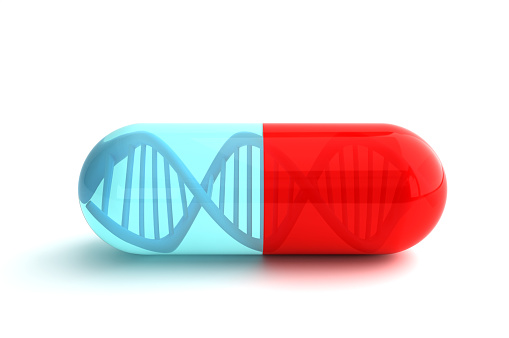
\includegraphics{pilldna}}\\[\baselineskip] % Publisher and logo
}}
\endgroup}

%----------------------------------------------------------------------------------------
%				BLANK DOCUMENT
%----------------------------------------------------------------------------------------

\begin{document}

\pagestyle{empty} % Removes page numbers

\titleGM % This command includes the title page


% ------------- TABLE OF CONTENTS -------------------

\tableofcontents

\newpage

% ----------------  SUMMARY PAGES ----------------------

\section{Patient haplotypes}

\scriptsize

\begin{tabularx}{\textwidth}{sbb}
\textbf{Gene} & \textbf{Phylogenetic method}\footnote{Method using phylogenetic trees to find closest 'relative' to patient alleles. Trees can be seen in Appendix A.} &  \textbf{Set method}\footnote{Method looking for overlap of haplotype non-reference variants and patient non-reference variants. Reference variants are filtered out of both sets prior to comparison. Top 5 hits can be seen in Appendix 2.}  \\
\hline \\

{{gene.symbol}} & {{gene.new1['1'] | replace("#", "\#") | replace("_", "-") }} / {{gene.new2['1'] | replace("#", "\#") | replace("_", "-") }} & {{gene.old1['1'] | replace("#", "\#") | replace("_", "-") }} / {{gene.old2['1'] | replace("#", "\#") | replace("_", "-") }} \\

\end{tabularx}

\normalsize

\newpage

\section{Drug annotations}
\begin{tabularx}{1.3\textwidth}{XXXX}
\textbf{Drug} & \textbf{Gene}  &  \textbf{Guideline} & \textbf{Annotations\footnote{ Level 1A and 1B clinical annotations meet the highest levels of criteria and are manually curated by PharmGKB. Level 1A annotations contain a variant-drug combination in a CPIC or medical society endorsed PGx guideline, or, implemented at a PGRN site, or, in another major health system. Level 1B annotations contain a variant-drug combination where the preponderance of evidence shows an association. The association must be replicated in more than one cohort with significant p-values, and, preferably with a strong effect size. Lower levels (3-4) are less significant and may only be based on a single study or case report, which may be performed in vitro.(PHARMGKB) }}  \\
\hline \\

{{item.drugname}} & {{item.gene}} & {{item.guid}} & \textit{Level 1-2}: {{item.annCount['1-2'] }} \newline \textit{Level 3-4}: {{item.annCount['3-4']}} \\

\end{tabularx}

\newpage

% ----------------  Guidelines ----------------------

\section{Haplotype Guidelines}




\subsection{ {{pair.drugname}} }
 - Empty description here -



\subsubsection{ {{pair.gene}} }

\begin{center}
Patient haplotype
\textbf{ {{pair.hapNEW}} } | \textbf{ {{pair.hapOLD}} } \newline\newline
\scriptsize
\begin{tabularx}{\textwidth}{ssbb}
{{pair.guideline.summary}}
\end{tabularx}

\end{center}



\newpage
\normalsize

% ----------------  High level Clinical Variations ----------------------


\section{Clinical Annotations}



\subsection{ {{drug.drugname}} }
{{drug.drugdesc}}



\subsubsection{ {{gene.symbol}} }

\begin{center}

\textbf{\colorbox{red} {Class 1A}} \textbf{ {{ann.rsid}} } \textit{ {{ann.patAllele}} }
{{ann.text}}


\textbf{\colorbox{orange} {Class 1B}} \textbf{ {{ann.rsid}} } \textit{ {{ann.patAllele}} }
{{ann.text}}


\textbf{\colorbox{yellow} {Class 2A}} \textbf{ {{ann.rsid}} } \textit{ {{ann.patAllele}} }
{{ann.text}}


\textbf{\colorbox{green} {Class 1A}} \textbf{ {{ann.rsid}} } \textit{ {{ann.patAllele}} }
{{ann.text}}





\end{center}



\newpage

% ----------------  APPENDICES ----------------------

\section{Appendix 1: Haplotype trees}
\begin{center}
\scriptsize

\textbf{ {{gene.symbol}} }
\begin{newicktree}
\nobranchlengths
\nonodemarkers
\righttree \setunitlength{0.5cm}
\drawtree{ {{gene.tree}} }\end{newicktree}

\normalsize
\end{center}

\newpage

\section{Appendix 2: Top 3 haplotypes per gene}

\begin{tabularx}{\textwidth}{ c c c c c }
test & \textbf{Allele 1 (Tree) } & \textbf{Allele 2 (Tree)} & \textbf{Allele 1 (Set) } & \textbf{Allele 2 (Set)} \\

\multirow{3}{200pt}{ {{gene.symbol}} } &
{{gene.new1.1}} & {{gene.new2.1}} & {{gene.old1.1}} & {{gene.old2.1}} \\
{{gene.new1.2}} & {{gene.new2.2}} & {{gene.old1.2}} & {{gene.old2.2}}  \\
{{gene.new1.3}} & {{gene.new2.3}} & {{gene.old1.3}} & {{gene.old2.3}} \\

\end{tabularx}

\section{Appendix 3: Low level annotations}



\subsection{ {{drug.drugname}} }
{{drug.drugdesc}}



\subsubsection{ {{gene.symbol}} }

\begin{center}

\textbf{\colorbox{cyan} {Class 3}} \textbf{ {{ann.rsid}} } \textit{ {{ann.patAllele}} }
{{ann.text}}


\textbf{\colorbox{blue} {Class 4}} \textbf{ {{ann.rsid}} } \textit{ {{ann.patAllele}} }
{{ann.text}}



No Annotations available.


\end{center}





% ------------------
\end{document}
